% Copyright 2004 by Till Tantau <tantau@users.sourceforge.net>.
%
% In principle, this file can be redistributed and/or modified under
% the terms of the GNU Public License, version 2.
%
% However, this file is supposed to be a template to be modified
% for your own needs. For this reason, if you use this file as a
% template and not specifically distribute it as part of a another
% package/program, I grant the extra permission to freely copy and
% modify this file as you see fit and even to delete this copyright
% notice. 

\documentclass[notes]{beamer}       % print frame + notes
%\documentclass[notes=only]{beamer}   % only notes
%\documentclass{beamer}              % only frames
%\documentclass[handout, notes=only]{beamer} % for printing notes
%\usepackage{handoutWithNotes}

% There are many different themes available for Beamer. A comprehensive
% list with examples is given here:
% http://deic.uab.es/~iblanes/beamer_gallery/index_by_theme.html
% You can uncomment the themes below if you would like to use a different
% one:
%\usetheme{AnnArbor}
%\usetheme{Antibes}
%\usetheme{Bergen}
%\usetheme{Berkeley}
%\usetheme{Berlin}
%\usetheme{Boadilla}
%\usetheme{boxes}
%\usetheme{CambridgeUS}
%\usetheme{Copenhagen}
%\usetheme{Darmstadt}
%\usetheme{default}
%\usetheme{Frankfurt}
%\usetheme{Goettingen}
%\usetheme{Hannover}
%\usetheme{Ilmenau}
%\usetheme{JuanLesPins}
%\usetheme{Luebeck}
\usetheme{Madrid}
%\usetheme{Malmoe}
%\usetheme{Marburg}
%\usetheme{Montpellier}
%\usetheme{PaloAlto}
%\usetheme{Pittsburgh}
%\usetheme{Rochester}
%\usetheme{Singapore}
%\usetheme{Szeged}
%\usetheme{Warsaw}

% Probability commands: Expectation, Variance, Covariance, Bias
\newcommand{\E}{\mathbb{E}}
\newcommand{\Var}{\mathrm{Var}}
\newcommand{\Cov}{\mathrm{Cov}}
\newcommand{\Bias}{\mathrm{Bias}}
\newcommand\indep{\protect\mathpalette{\protect\independenT}{\perp}}
\def\independenT#1#2{\mathrel{\rlap{$#1#2$}\mkern2mu{#1#2}}}

\title{Two Papers on Sparse Feature Selection in Multivariate Regression}

% A subtitle is optional and this may be deleted
%\subtitle{Optional Subtitle}

\author{Gregory Faletto}
%\author{F.~Author\inst{1} \and S.~Another\inst{2}}
% - Give the names in the same order as the appear in the paper.
% - Use the \inst{?} command only if the authors have different
%   affiliation.

\institute[USC Marshall] % (optional, but mostly needed)
{
%  \inst{1}%
  Department of Data Sciences and Operations\\
  Statistics Group \\
  University of Southern California Marshall School of Business}
%  \and
%  \inst{2}%
%  Department of Theoretical Philosophy\\
%  University of Elsewhere}
% - Use the \inst command only if there are several affiliations.
% - Keep it simple, no one is interested in your street address.

\date{DSO 607, April 1 2019}
% - Either use conference name or its abbreviation.
% - Not really informative to the audience, more for people (including
%   yourself) who are reading the slides online

%\subject{Theoretical Computer Science}
% This is only inserted into the PDF information catalog. Can be left
% out. 

% If you have a file called "university-logo-filename.xxx", where xxx
% is a graphic format that can be processed by latex or pdflatex,
% resp., then you can add a logo as follows:

% \pgfdeclareimage[height=0.5cm]{university-logo}{university-logo-filename}
% \logo{\pgfuseimage{university-logo}}

% Delete this, if you do not want the table of contents to pop up at
% the beginning of each subsection:
\AtBeginSubsection[]
{
  \begin{frame}<beamer>{Outline}
    \tableofcontents[currentsection,currentsubsection]
  \end{frame}
}

%\pgfpagesuselayout{4 on 1 with notes}[a4paper,border shrink=5mm]

% Let's get started
\begin{document}

\begin{frame}
  \titlepage
\end{frame}

\begin{frame}{Outline}
  \tableofcontents
  % You might wish to add the option [pausesections]
\end{frame}



\section{Background on Multivariate Regression}

%\subsection{Another Subsection}
%
%\begin{frame}{Blocks}
%\begin{block}{Block Title}
%You can also highlight sections of your presentation in a block, with it's own title
%\end{block}
%\begin{theorem}
%There are separate environments for theorems, examples, definitions and proofs.
%\end{theorem}
%\begin{example}
%Here is an example of an example block.
%\end{example}
%\end{frame}

\begin{frame}{Setup and Notation for Multivariate Linear Regression (single observation)}{}
\begin{center}
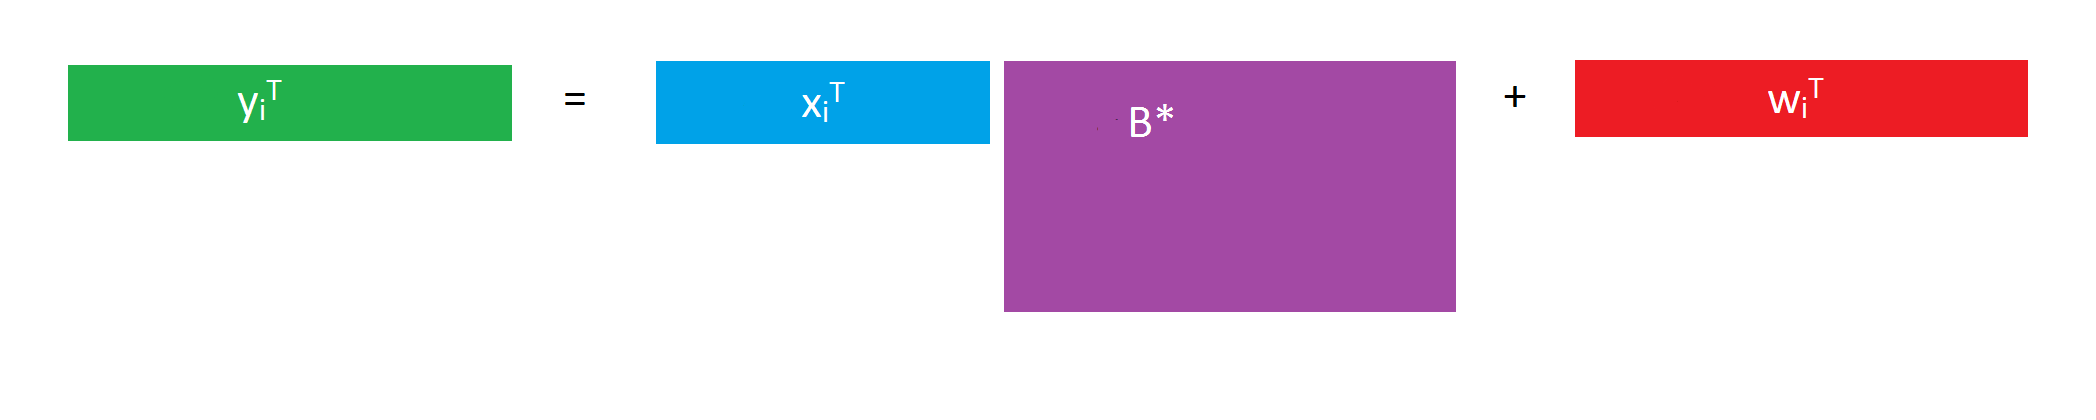
\includegraphics[scale=0.22]{diagram1.png}
\end{center}
\end{frame}

\begin{frame}{Setup and Notation for Multivariate Linear Regression (single observation)}{}



     Formulation for individual response \(\boldsymbol{y}_i \):

\begin{equation}
\underbrace{\boldsymbol{y}_i^T}_{ 1 \times K} = \underbrace{\boldsymbol{x}_i^T}_{1 \times p} \underbrace{\boldsymbol{B}^*}_{p \times K} + \underbrace{\boldsymbol{w}_i^T}_{1 \times K}
\end{equation}

where

\begin{itemize}

\item \(\boldsymbol{y}_i \in \mathbb{R}^K\) is a \(K\)-vector of responses (rather than a scalar response as in univariate linear regression),

\item \(\boldsymbol{x}_i \in \mathbb{R}^p\) is a \(p\)-vector of predictors associated with \(\boldsymbol{y}_i\) (same as in univariate regression),

\item \(\boldsymbol{B}^* \in \mathbb{R}^{p \times K}\) is a \(p \times K\) matrix of coefficients (rather than a \(p\)-vector of coefficients as in univariate regression),

\item \(\boldsymbol{w}_i \in \mathbb{R}^K\) is a \(K\)-vector of random errors.

\end{itemize}

\end{frame}

\begin{frame}{Setup and Notation for Multivariate Linear Regression (full data set)}{}
\begin{center}
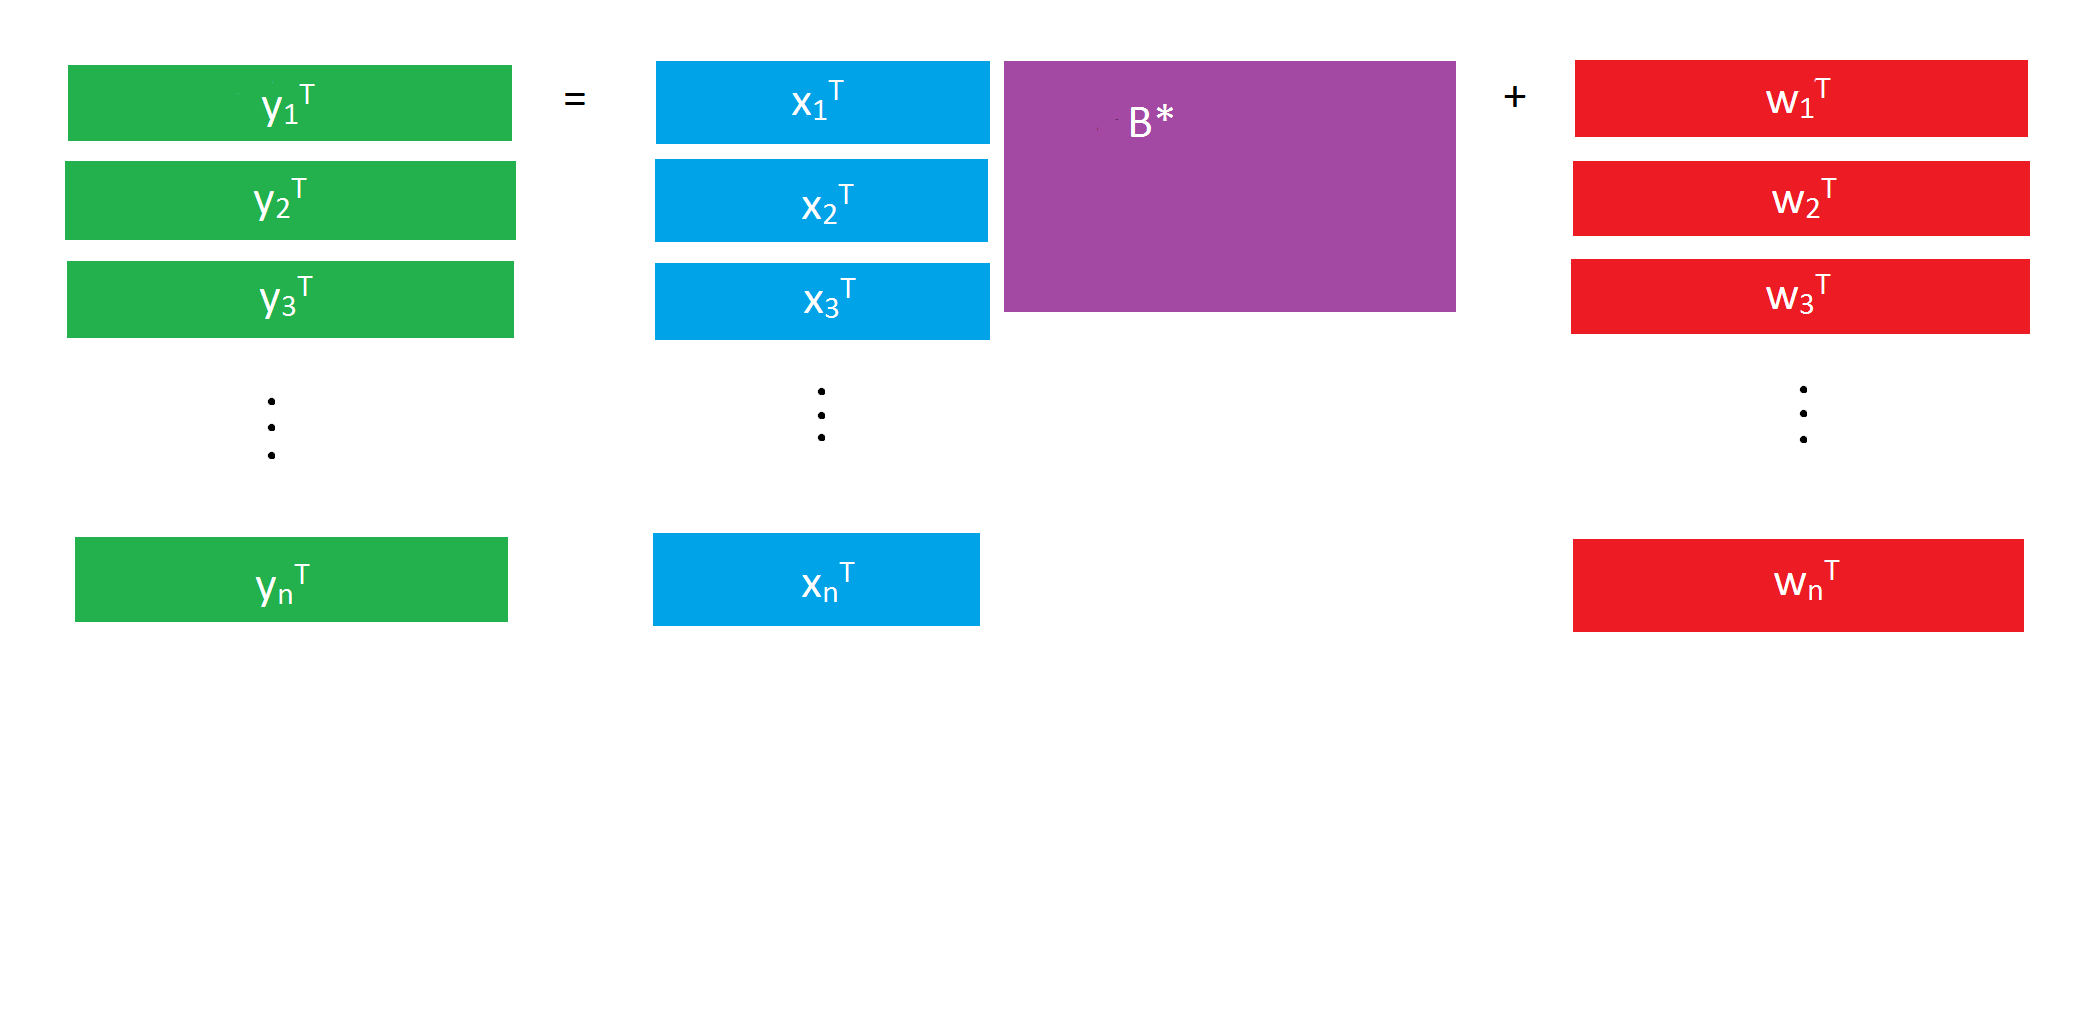
\includegraphics[scale=0.22]{diagram2.png}
\end{center}
\end{frame}


\begin{frame}{Setup for Multivariate Linear Regression (full data set)}{}

   Formulation for full data set:

\begin{equation}
\underbrace{\boldsymbol{Y}}_{n \times K} = \underbrace{\boldsymbol{X}}_{n \times p} \underbrace{\boldsymbol{B}^*}_{p \times K} + \underbrace{\boldsymbol{W}}_{n \times K}
\end{equation}
  
  where

\begin{itemize}

\item \(\boldsymbol{Y} \in \mathbb{R}^{n \times K} = (\boldsymbol{y}_1, \ldots, \boldsymbol{y}_n)^T\) is an \(n \times K\) matrix of responses (row \(i\) contains response \(\boldsymbol{y}_i\)),

\item \(\boldsymbol{X} \in \mathbb{R}^{n \times p}\) is an \(n \times p\) matrix of predictors (same as in univariate regression),

\item \(\boldsymbol{B}^* \in \mathbb{R}^{p \times K}\) is a \(p \times K\) matrix of coefficients,

\item \(\boldsymbol{W} \in \mathbb{R}^{n \times K} = (\boldsymbol{w}_i, \ldots, \boldsymbol{W}_n)^T\) is an \(n \times K\) matrix of random errors. The error vectors are assumed to be IID with \(\E(\boldsymbol{w}_i) = \boldsymbol{0}\).

\end{itemize}

\end{frame}

\begin{frame}{Some Motivating Examples}{}
  \begin{itemize}
  \item Predicting both Math and Verbal SAT score as a function of parental income, extracurricular activity participation, etc.
  \item Responses of several measures of health to a drug in the presents of other covariates (age, weight, gender, etc.)
  \item Prediction of the prices of several stocks as a function of economic indicators
  \item Used to find sets of genes that are expressed in different forms of cancer in Chen, Chan, and Stenseth (2012)
  \end{itemize}
  
  \end{frame}
  
  \note[itemize]{
  \item Sometimes called ``multi-task learning" in machine learning
  \item Won't go through example of gene expression because it's a different paradigm from the usual case we'll discuss
  }


% Section and subsections will appear in the presentation overview
% and table of contents.
\section{Support Union Recovery in High-Dimensional Multivariate Regression (Obozinski, Wainwright, and Jordan 2011)}

\subsection{Background and Problem Statement}

\begin{frame}{Meaning of ``Support Union Recovery"}{}
  \begin{itemize}
  \item {
    Feature selection in multivariate setting
  }
  \item {
   Sparsity assumption: column \(k\) of coefficient matrix \(\boldsymbol{B}^*\) has nonzero entries in a subset
   
   \begin{equation}
   S_k := \{i \in \{1, \ldots, p \} \mid \beta_{ik}^* \neq 0 \}
   \end{equation}
   
   of size \(s_k := | S_k|\).
  }


  \item{We seek to \textit{recover} the \textit{union} of the \textit{supports}: the set 
  
  \[
  S := \bigcup_{k=1}^K S_k
  \]
  }
  
  of size \(s:= |S|\).
  \end{itemize}
\end{frame}

\note[itemize]{
  \item{Responses are related, so we expect supports \(S_k\) should have some overlap, and that the relationship between the supports and responses (i.e. the coefficients, or the vectors in the columns of \(\boldsymbol{B}\) are related).
  
  }
}

\begin{frame}{Block Regularization}{}
  \begin{itemize}
  \item {
    Used in many settings when goal is to choose whether or not to include groups of variables, rather than considering them individually.
  }
%  \item {
%   Example: \(\ell_0/\ell_q\) norm of a matrix counts the number of rows with nonzero \(\ell_q\) norm.
%   
%
%  }

  \item{Example: \(\ell_1/\ell_q\) norm of a matrix takes the sum of the \(\ell_q\) norms of each row:
  
  \begin{equation}
  \lVert \boldsymbol{B} \rVert_{\ell_1/\ell_q} := \sum_{i=1}^p \Bigg( \sum_{j=1}^K |\beta_{ij}|^q \Bigg)^{1/q} = \sum_{i=1}^p \lVert \beta_i \rVert_q
  \end{equation}
  
  where \((\beta_{ik})_{1 \leq i \leq p, 1 \leq k \leq K}\) are the entries of \(\boldsymbol{B}\).
  
  }
  \item{This paper makes use of the \(\ell_1/\ell_2\) norm
  
    \begin{equation}
  \lVert \boldsymbol{B} \rVert_{\ell_1/\ell_2} := \sum_{i=1}^p \sqrt{ \sum_{j=1}^K \beta_{ij}^2 } = \sum_{i=1}^p \lVert \beta_i \rVert_2
  \end{equation}
  }
  \end{itemize}
\end{frame}

\begin{frame}{Multivariate Group Lasso}{}
  \begin{itemize}
  \item{We solve the following optimization problem to estimate \(\boldsymbol{B}^*\):
   
   \begin{equation}\label{linreg.pres.mult.group.lasso.opt.problem}
   \underset{\boldsymbol{B} \in \mathbb{R}^{p \times K}} {\arg \min}\left\{  \frac{1}{2n} \lVert \boldsymbol{Y} - \boldsymbol{X} \boldsymbol{B} \rVert_F^2 + \lambda_n \lVert \boldsymbol{B} \rVert _{\ell_1/\ell_q}\right\}
   \end{equation}
   
   where \(\lVert \cdot \rVert_F\) denotes the Frobenius norm:
   
   \[
   \lVert A \rVert_F := \sqrt{ \sum_{i,j} A_{i,j}^2}.
   \]
  }


  \item{Penalizing the \(\ell_1/\ell_1\) norm is equivalent to simply solving \(K\) separate lasso solutions.
  

  }
  \item{Penalizing the \(\ell_1/\ell_2\) nor groups rows together; the authors call this the \textbf{multivariate group lasso}.
  }
  \end{itemize}
\end{frame}

\note[itemize]{
    \item {Note that when \(K=1\) this is exactly the lasso (regardless of \(q\)):
    
     \begin{equation}
  \lVert \boldsymbol{B} \rVert_{\ell_1/\ell_1} := \sum_{i=1}^p \Bigg( \sum_{j=1}^K |\beta_{ij}|^1 \Bigg)^{1/1} = \sum_{i=1}^p | \beta_i |
  \end{equation}

  }
  \item When \(q=1\) the sum decouples (show on board)
}

\begin{frame}{Multivariate Group Lasso (continued)}{}
  \begin{itemize}
  \item{The Frobenius norm is convex; therefore the optimization problem (\ref{linreg.pres.mult.group.lasso.opt.problem}) is convex and can be solved efficiently. (In particular, it is a second-order cone program (SOCP) and can be solved efficiently with interior point methods.)
  
  \begin{equation}\tag{\ref{linreg.pres.mult.group.lasso.opt.problem}}
   \underset{\boldsymbol{B} \in \mathbb{R}^{p \times K}} {\arg \min}\left\{  \frac{1}{2n} \lVert \boldsymbol{Y} - \boldsymbol{X} \boldsymbol{B} \rVert_F^2 + \lambda_n \lVert \boldsymbol{B} \rVert _{\ell_1/\ell_q}\right\}
   \end{equation}
  }

  \end{itemize}
\end{frame}



\begin{frame}{Main Assumptions}{}
  \begin{itemize}
  \item {
    (A1) \textit{Bounded eigenspectrum:} There exist fixed constants \(C_{\text{min}} > 0\) and \(C_{\text{max}} < + \infty\) such that all eigenvalues of the \(s \times s\) matrix \(\Sigma_{SS}\) (the covariance matrix of the true support) are contained in the interval \([C_{\text{min}}, C_{\text{max}}]\). 
%    \pause % The slide will pause after showing the first item
  }
  \item {
    (A2) \textit{Irrepresentable Condition:} There exists a fixed parameter \(\gamma \in (0,1]\) such that
    
    \[
    \lVert \Sigma_{S^CS} \big( \Sigma_{SS} \big)^{-1} \rVert_{\infty} \leq 1 - \gamma.
    \]
    
   
%    \pause % The slide will pause after showing the first item
  }
  % You can also specify when the content should appear
  % by using <n->:
%  \item<3-> {
  \item {
    (A3) \textit{Self-incoherence:} There exists some \(D_{\text{max}} < + \infty\) such that
    
    \[
      \lVert \big( \Sigma_{SS} \big)^{-1} \rVert_{\infty} \leq D_{\text{max}}.
    \]
    
  
%    \pause % The slide will pause after showing the first item
  }
  \end{itemize}
\end{frame}

\note[itemize]{
    \item {Intuition of bounded eigenspectrum condition: prevents excess dependence among elements of the design matrix associated with the support \(S\).)

  }
  \item  Intuition of Irrepresentable condition: correlation between features in true support and noise features is not too high.
}

\begin{frame}{Sparsity Overlap function}{}
  \begin{itemize}
  \item{\textit{Sparsity-overlap function} \(\phi(\boldsymbol{B}^*) \) measures the sparsity of the matrix \(\boldsymbol{B}^*\) as well as the overlap between the different regressions (the different columns of \(\boldsymbol{B}^*\)).
 }

  \item{In case of univariate regression \(K=1\), entries of design matrix are i.i.d.  standard Gaussian; then \(\phi(\boldsymbol{B}^*)=s\).
  }
  \item{For suitably correlated designs: sparsity overlap is  \(\phi(\boldsymbol{B}^*)=s/K\).
  }
  \item{Lemma 1(a): Under assumption (A1), the sparsity overlap \(\phi(\boldsymbol{B}^*)\) obeys the bounds
  
  \[
  \frac{s}{C_{\text{max}}K} \leq \phi(\boldsymbol{B}^*) \leq \frac{s}{C_{\text{min}}}.
  \]
  }


  \end{itemize}
\end{frame}

\note[itemize]{
\item We will see in Theorem 1 (next slide) that when the sparsity overlap is small, multivariate group lasso performs more favorably. Therefore we want \(C_{min}\) to be large (not too close to 0, hopefully close to 1).
}

\subsection{Main Results}

% You can reveal the parts of a slide one at a time
% with the \pause command:


\begin{frame}{Main Results}{(under assumptions A1 - A3 and some other mild conditions)}
  \begin{itemize}
  \item {
    (Summary of Theorem 1.) The \textit{sample complexity}
    
    \[
    \theta(n,p,s):= \frac{n}{2 \psi(\boldsymbol{B}^*) \log(p - s)},
    \]
    
    determines whether the multivariate group lasso recovers the exact row pattern (with high probability).
    
%    where \( \psi(\boldsymbol{B}^*)\) is a sparsity-overlap function 
%    \pause % The slide will pause after showing the first item
  }
    \item{
    (Summary of Corollary 1.) In particular, in the special case of the standard Gaussian ensemble, if \(\theta(n, p, s)\) exceeds a critical level \(\theta\), the multivariate group lasso has a unique solution \(\hat{\boldsymbol{B}}\) with row support \(S(\boldsymbol{B})\) that is contained within the true row support \(S(\boldsymbol{B}^*)\). Additionally, \(\lVert \hat{\boldsymbol{B}} - \boldsymbol{B}^* \rVert_{\ell_\infty/\ell_2}\) is bounded. If \(\theta(n, p, s)\) is below the critical level \(\theta\), the multivariate group lasso fails.
  }
\item {   
    More generally, the multivariate group lasso succeeds for problem sequences \((n, p, s)\) such that \(\theta(n, p, s)\) exceeds a critical level \(\theta_u\) and fails for sequences such that \(\theta(n, p, s)\) lies below a critical level \(\theta_{\ell}\).
  }

  % You can also specify when the content should appear
  % by using <n->:
%  \item<3-> {

  
   
  \end{itemize}
\end{frame}

% You can reveal the parts of a slide one at a time
% with the \pause command:
\begin{frame}{Main Results (continued)}{(under assumptions A1 - A3 and some other mild conditions)}
  \begin{itemize}
  \item{Recall Lemma 1(a): under assumption (A1) we have bounds on \(\phi(\boldsymbol{B}^*)\), so \( \theta(n,p,s)\) ranges between
  \begin{equation}\label{linreg.pres.mult.group.lasso.complexity.range}
     \frac{nC_{\text{min}}}{2 s\log(p - s)} \leq   \theta(n,p,s) \leq  \frac{nC_{\text{max}}K}{2 s\log(p - s)} .
   \end{equation}
  
This generalizes a previous result from Wanwright (2009): the lasso succeeds in performing exact support recovery if the ratio \(n/[s \log(p-s)]\) exceeds a certain threshold.
}
   
  \item{
%  \item<4-> {
    (Summary of Corollary 3 and part of Corollary 1.) If \(\boldsymbol{X}\) is uncorrelated for the variables corresponding to the active rows of \(\boldsymbol{B}^*\), \(\ell_1/\ell_2\) group regularization never harms performance relative to an ordinary lasso approach.
  }
  % or you can use the \uncover command to reveal general
  % content (not just \items):

  \end{itemize}
\end{frame}


\note[itemize]{
%    \item {The quantity on the left side of (\ref{linreg.pres.mult.group.lasso.complexity.range}) shows that 
%
%  }
%  \item From the sparsity-overlap function \( \psi(\boldsymbol{B}^*)\), we learn that 
	\item  Per (\ref{linreg.pres.mult.group.lasso.complexity.range}), \(\ell_1/\ell_2\) regularization for multivariate regression can yield substantial improvements in sample complexity (up to a factor of \(K\)) when the coefficient vectors are suitably orthogonal. 
}


\begin{frame}{Main Results (continued)}{(under assumptions A1 - A3 and some other mild conditions)}
%  \begin{itemize}
% \item{
    (Summary of Corollary 2.) Given a method that returns the row supports \(S\) (with high probability) with \(|S| \ll p\), recovering the individual supports \(S_k\) with high probability is easy using the following procedure:
    \begin{enumerate}[(1)]
    \item Compute the (restricted) multivariate ordinary least squares estimate
    
    \begin{equation}
    \tilde{\boldsymbol{B}}_{\hat{S}} = \underset{\boldsymbol{B}_{\hat{S}}}{ \arg \min} \left\{   \lVert \boldsymbol{Y} - \boldsymbol{X}_{\hat{S}} \boldsymbol{B}_{\hat{S}} \rVert_F \right\}
    \end{equation}
    
    where \( \boldsymbol{B}_{\hat{S}}\) is the coefficient matrix \(\boldsymbol{B}\) but only with rows in the estimated support union \(\hat{S}\) and  \( \boldsymbol{X}_{\hat{S}}\) contains only the columns of \(\boldsymbol{X}\) corresponding to those features.
    
    \item Compute \(T(\tilde{\boldsymbol{B}}_{\hat{S}})\) by setting every entry in \( \tilde{\boldsymbol{B}}_{\hat{S}} \) with absolute value less than \(2 \sqrt{ 2 \log(K |\hat{S}|)/(C_{\text{min}} n}\) equal to 0. Then the support is the nonzero entries of \(T(\tilde{\boldsymbol{B}}_{\hat{S}})\).
    
    \end{enumerate}
%  }
  % or you can use the \uncover command to reveal general
  % content (not just \items):
%  \item{
%%  \item<5-> {
%    In more general designs, it is possible for the ordinary lasso to outperform the multivariate group lasso. 
%%    \uncover<6->{Extra text in the fifth item.}
%  }
%    \item<5-> {
   
%  \end{itemize}
\end{frame}

%\note[itemize]{
%\item By ``ordinary lasso" I mean fitting lasso on each response separately and combining these support estimates to estimate the support union)
%}

\subsection{Selected Simulation Studies}

\begin{frame}
\begin{center}
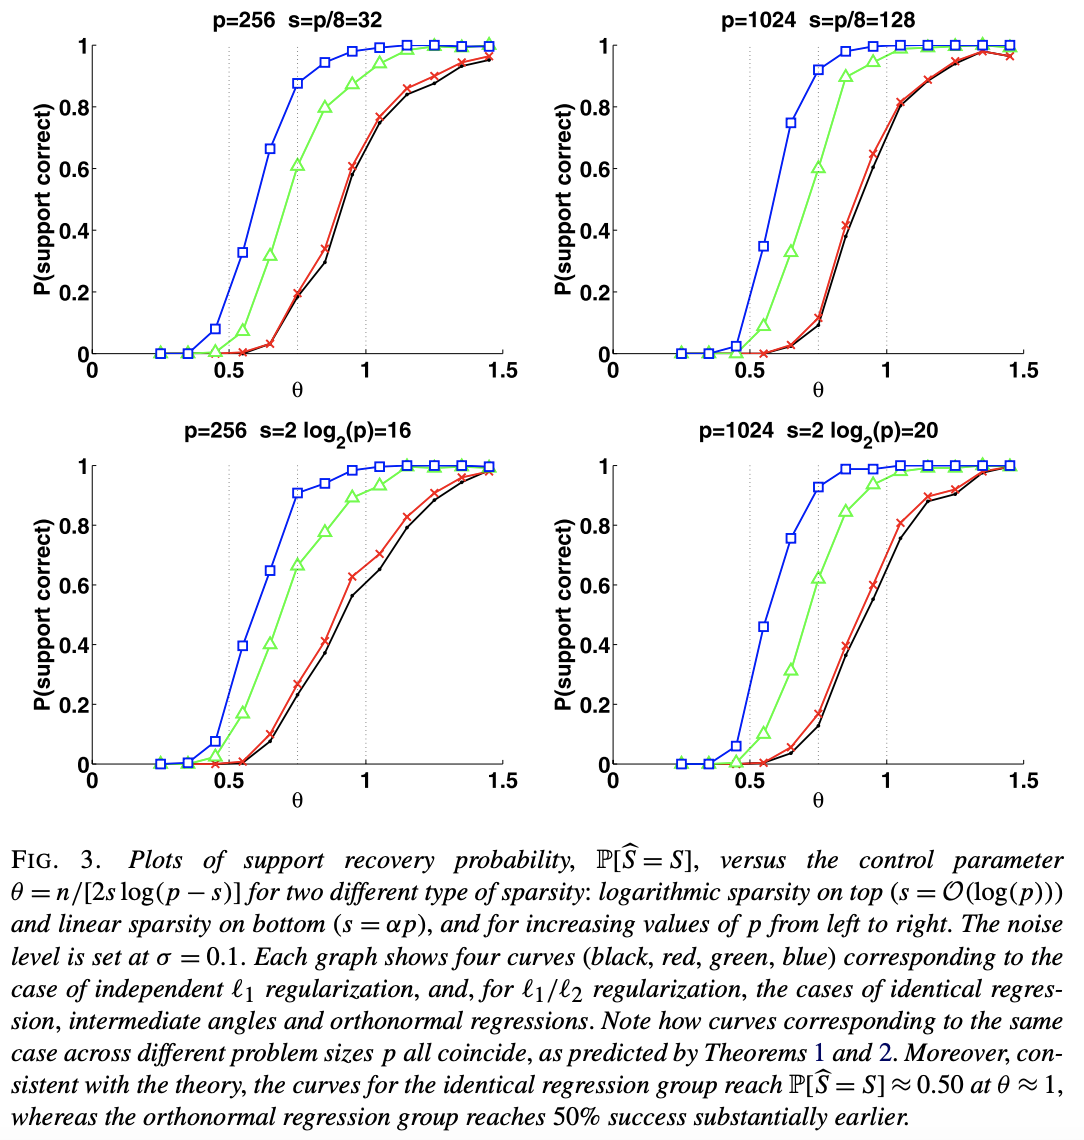
\includegraphics[scale=0.4]{fig3a.png}
\end{center}
\end{frame}

\note[itemize]{
\item This illustrates threshold effect predicted by Theorems 1 and 2. Case of 2 responses (\(K=2\)) which share an identical support set \(S\) with cardinality \(s\) (so \(\boldsymbol{B}^*\)  is an \(s \times 2\) matrix).
\item Fixed regularization parameter 

\[
\lambda_n = \sqrt{\frac{\log(p-s) \log(s) }{n}}. 
\]

Move across independent axis by varying \(\theta\) (\(p\) fixed, \(s\) determined by ratio or logarithm)
\item In all cases here, design matrix is sampled from standard Gaussian ensemble. What we see here is that the probability of support recovery increases with the control parameter 

\[
\theta = \frac{n}{2s \log(p-s)}.
\]

}

\note[itemize]{
\item Black curve is independent \(\ell_1\) regularization (ordinary lasso), which we see does the worst in pretty much all settings. Red is \(\ell_1/\ell_2\) regularization for identical regression (the columns of \(\boldsymbol{B}^*\) are identical). For orthonormal regressions (blue lines), the columns of \(\boldsymbol{B}^*\) are orthonormal, which is the most favorable setting for this method. For intermediate angles (green lines), the columns of \(\boldsymbol{B}^*\) are at a 60 degree angle.

\item Note that the improvement of this method over lasso is largest when the regressions are orthonormal; in the other extreme when the columns are identical, it does about the same as lasso.

\item Note that varying \(p\) doesn't really change anything if the control parameter \(\theta\) is equal.

\item In identical regression group, \(\Pr\) support recovery reaches 0.5 at \(\theta=1\); improvement in other regimes.
}

\begin{frame}
\begin{center}
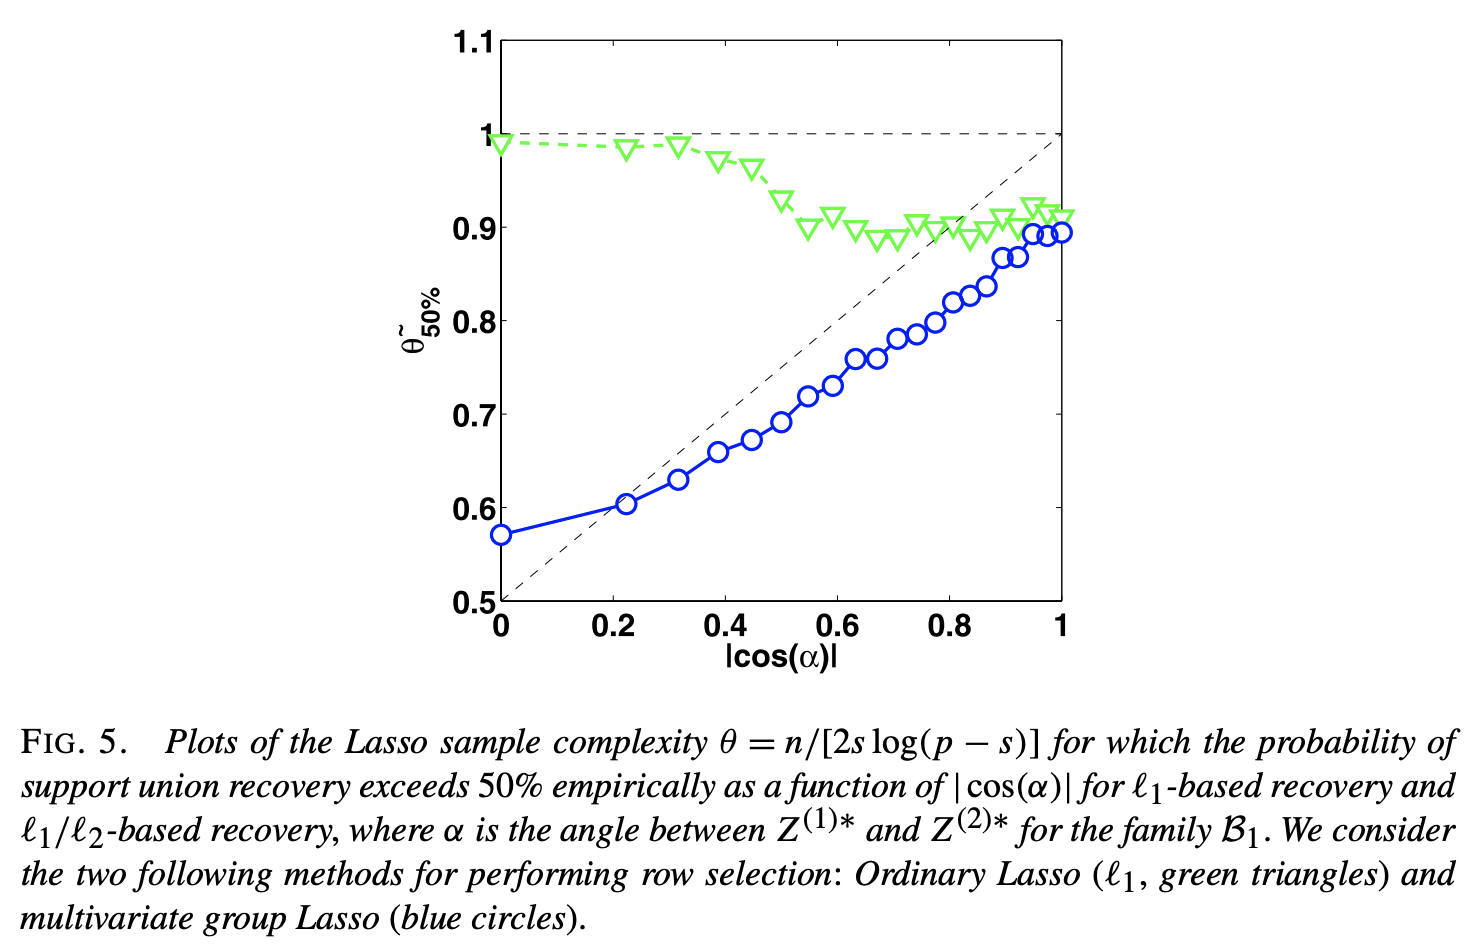
\includegraphics[scale=0.48]{fig5a.png}
\end{center}
\end{frame}

\note[itemize]{
\item We have fixed \(p = 2048\) and sparsity \(s = \log_2 (p) = 22\).
\item \(\alpha\) is the angle between columns of  \(\boldsymbol{B}^*\), so as its cosine increases, the columns come closer together.
\item We see that lasso needs a higher value of \(\theta\) to get a \(50\%\) chance of support recovery, but the gap decreases as the columns of \(\boldsymbol{B}^*\) come closer and closer together, until there is no gap when they are equal.
\item Theory from this paper predicts that the circles and triangles should lie at or below dotted lines.
\item Intuition of why this method does better when columns are orthonormal: in that case independent estimates of the support are more likely to include (by union) spurious covariates in the row support.
}

%\begin{frame}{First Slide Title}{Optional Subtitle}
%  \begin{itemize}
%  \item {
%    My first point.
%  }
%  \item {
%    My second point.
%  }
%  \end{itemize}
%\end{frame}


\section{Reduced Rank Stochastic Regression with a Sparse Singular Value Decomposition (Chen, Chan, and Stenseth 2012)}

\subsection{Background and Problem Statement}

\begin{frame}{Singular Value Decomposition of the coefficient matrix \( \boldsymbol{B}^*\)}
  \begin{itemize}
 \item{
    Reduced rank regression model: \(\boldsymbol{Y} = \boldsymbol{X} \boldsymbol{B}^* + \boldsymbol{W}\) as before. We will be concerned with \(\operatorname{rank}(\boldsymbol{B}^*) = r^* \leq \min \{p, K\}\).
    
%\begin{equation}\label{linreg.pres.reduced.rank.model}

%\end{equation}


    
  }
%    \item{
% The rank \(r\) least squares estimator of \(\boldsymbol{B}^*\) that minimizes \(\lVert \boldsymbol{Y}  - \boldsymbol{X} \boldsymbol{B}^* \rVert_F^2\) subject to \(\operatorname{rank}(\boldsymbol{B}^*) = r\) can be obtained explicitly (Reinsel and Velu 1998).
%%    \uncover<6->{Extra text in the fifth item.}
%  }

  \item{Singular value decomposition (SVD):
  
  \begin{equation}\label{linreg.pres.reduced.rank.svd.sum}
\boldsymbol{B}^* = \boldsymbol{U} \boldsymbol{D} \boldsymbol{V}^T = \sum_{k=1}^{r^*} d_k \boldsymbol{u}_k\boldsymbol{v}_k^T = \sum_{k=1}^{r^*} \boldsymbol{B}_k
\end{equation}
  }
  
  \begin{itemize}
  \item \(\boldsymbol{U}  = (\boldsymbol{u}_1, \ldots, \boldsymbol{u}_{r^*}) \in \mathbb{R}^{p \times r^*}\) consists of orthonormal left singular vectors
  \item \(\boldsymbol{V}  = (\boldsymbol{v}_1, \ldots, \boldsymbol{v}_{r^*}) \in \mathbb{R}^{K \times r^*}\) consists of orthonormal right singular vectors
  \item \(\boldsymbol{D} \in \mathbb{R}^{r^* \times r^*}\) is a diagonal matrix with positive singular values \(d_1 > \ldots, > d_{r^*}\) on its diagonal. 
  \end{itemize} 



  % or you can use the \uncover command to reveal general
  % content (not just \items):
  
    \end{itemize}
\end{frame}


\note[itemize]{
\item  Using singular value decomposition, \( \boldsymbol{B}^*\) can be expressed as a sum of \(r^*\) unit rank matrices \(\boldsymbol{B}_k\) that are proportional to the outer product of the left and right singular vectors.
\item (The singular values are assumed to be distinct, so the decomposition is unique up to the signs of the singular vectors. In practice this is usually the case.)
}


\begin{frame}{Singular Value Decomposition of \( \boldsymbol{B}^*\) (continued)}
  \begin{itemize}

%    \item<5-> {
   \item{\textbf{Key insight:} \( \boldsymbol{B}^*\) is the sum of \(r^*\) orthogonal layers of decreasing importance. For each layer \(k\), \(\boldsymbol{u}_k\) are the predictor effects, \(\boldsymbol{v}_k\) are the response effects, and \(d_k\) indicates the relative importance of the association.
   }
   \item{If we believe that each pathway of association involves only a subset of the responses and predictors, then the left and right singular vectors should be sparse.
   }
  \end{itemize}
\end{frame}

\subsection{Optimization Problem}

\begin{frame}{Optimization Problem}
%  \begin{itemize}

%    \item<5-> {
%   \item{ 
   We plug the expression for \( \boldsymbol{B}^*\) from (\ref{linreg.pres.reduced.rank.svd.sum}) into the typical penalized least squares objective function (similar to (\ref{linreg.pres.mult.group.lasso.opt.problem})) to obtain the objective function to optimize:
   
   \begin{equation}\label{linreg.pres.reduced.rank.svd.opt.problem}
    \underset{d_k, \boldsymbol{u}_k, \boldsymbol{v}_k, k \in 1, \ldots, r^*}{\arg \min} \left\{ \frac{1}{2} \left\lVert \boldsymbol{Y} - \boldsymbol{X} \sum_{k=1}^{r^*} d_k  \boldsymbol{u}_k, \boldsymbol{v}_k^T \right\rVert_F^2 + \sum_{k=1}^{r^*} p_\lambda \big( \lambda_k, (d_k, \boldsymbol{u}_k, \boldsymbol{v}_k) \big) \right \}
    \end{equation}
    where \(p_\lambda\) is a penalty function (to be specified), \( \lVert  \boldsymbol{u}_k \rVert_2 = 1\) and \( \lVert \boldsymbol{v}_k \rVert_2 = 1\).
%   }
 
%  \end{itemize}
\end{frame}

\begin{frame}{Optimization Problem}{Penalty Function}
  \begin{itemize}
    \item{The penalty function used to encourage sparsity is 
   
   \[
   p_\lambda \big( \lambda_k, (d_k, \boldsymbol{u}_k, \boldsymbol{v}_k) \big) = \lambda_k \sum_{i=1}^p \sum_{j=1}^K w_{ijk} |d_k u_{ik} v_{jk} | 
   \]
   \begin{equation}\label{linreg.pres.reduced.rank.svd.penalty}
   = \lambda_k (w_k^{(d)} d_k) \Bigg( \sum_{i=1}^p w_{ik}^{(u)} |u_{ik}| \Bigg)\Bigg( \sum_{j=1}^K w_{jk}^{(v)} |v_{jk}| \Bigg)
   \end{equation}
   }
   \item{Penalizes each singular vector in the SVD layer, creating automatic adjustment of sparsity between \( \boldsymbol{u}_k\) and \(\boldsymbol{v}_k\).
   }
   
   \item{ \(w_{ijk}\) is a weighting term (similar to the adaptive lasso (Zou 2006))
   }
  \end{itemize}
\end{frame}

\note[itemize]{
\item Weight term allows for flexibility in how much we penalize individual terms in each SVD layer.
}

%\begin{frame}{Optimization Problem}{Penalty Function}
%  \begin{itemize}
%    \item{The penalty function used to encourage sparsity is 
%   
%   \[
%   p_\lambda \big( \lambda_k, (d_k, \boldsymbol{u}_k, \boldsymbol{v}_k) \big) = \lambda_k \sum_{i=1}^p \sum_{j=1}^K w_{ijk} |d_k u_{ik} v_{jk} | 
%   \]
%   \begin{equation}\label{linreg.pres.reduced.rank.svd.penalty}
%   = \lambda_k (w_k^{(d)} d_k) \Bigg( \sum_{i=1}^p w_{ik}^{(u)} |u_{ik}| \Bigg)\Bigg( \sum_{j=1}^K w_{jk}^{(v)} |v_{jk}| \Bigg)
%   \end{equation}
%   }
%   \item{The penalty function penalizes each of the singular vectors in the SVD layer, creating automatic adjustment of sparsity between \( \boldsymbol{u}_k\) and \(\boldsymbol{v}_k\).
%   }
%   
%   \item{Somewhat similarly to the adaptive lasso (Zou 2006), we have an extra term \(w_{ijk} \) that allows for flexibility in how much we penalize individual terms in each SVD layer.
%   }
%  \end{itemize}
%\end{frame}

\begin{frame}{Adaptive Lasso (review)}
  \begin{itemize}
  \item{Recall from Zou (2006): adaptive lasso estimates \(\hat{\boldsymbol{\beta}}^{*(n)}\) are given by
  \begin{equation}
  \hat{\boldsymbol{\beta}}^{*(n)} =\underset{\boldsymbol{\beta \in \mathbb{R}^p}}{\arg \min}   \left\{\left\lVert \boldsymbol{y} - \boldsymbol{X}\boldsymbol{\beta} \right\rVert_2^2 + \lambda_n \sum_{j=1}^p \hat{w}_j | \beta_j| \right\}
  \end{equation}
  where \(\hat{\boldsymbol{w}} = (|\hat{\beta}_1|^{-2},  \ldots, |\hat{\beta}_p|^{-2}) \) where \(\hat{\boldsymbol{\beta}} = (\hat{\beta}_1, \ldots, \hat{\beta_p})\) is the OLS estimate for \(\beta\).
  }
  \item{Zou shows the adaptive lasso is consistent in variable selection and that the asymptotic distribution of \( \hat{\boldsymbol{\beta}}^{*(n)} \) is normal, unbiased, and efficient. 
  }


  \end{itemize}
\end{frame}

\note[itemize]{
\item  in the (univariate) linear model \(\boldsymbol{y} = \boldsymbol{X}\boldsymbol{\beta} + \boldsymbol{\epsilon}\)
\item (We will see that CCS prove similar results for their estimator.)
}

\begin{frame}{Optimization Problem}{Penalty Function (continued)}
  \begin{itemize}
  \item{In the rank one case (\(r^*=1\), so we don't index over \(k\)), Chen, Chan and Stenseth (CCS) choose the penalty weightings \(w^{(d)}, \boldsymbol{w}^{(u)}, \boldsymbol{w}^{(v)}\) in (\ref{linreg.pres.reduced.rank.svd.penalty}) as follows:
  \begin{enumerate}
  \item Estimate \(\boldsymbol{B}^*\) (call the estimate \(\tilde{\boldsymbol{B}}\))
  \item Find the SVD of \(\tilde{\boldsymbol{B}}\): \(\tilde{\boldsymbol{B}} = \tilde{d}\tilde{\boldsymbol{u}}\tilde{\boldsymbol{v}}^T \)
  \item Set 
  \begin{equation}
  \begin{cases}
  w^{(d)} = |\tilde{d}|^{-2} \\
   \boldsymbol{w}^{(u)} = (|\tilde{u}_1|^{-2}, \ldots, |\tilde{u}_p|^{-2}) \\
    \boldsymbol{w}^{(v)} =   (|\tilde{v}_1|^{-2}, \ldots, |\tilde{v}_K|^{-2})
  \end{cases}
  \end{equation}
  \end{enumerate}
  
  }

  \item{CCS provide a (more complicated) generalization of this rule for the general case (\(r^* \in \mathbb{N}\)).
  }
  
    \end{itemize}
\end{frame}

\note[itemize]{
\item Note the similarity to the adaptive lasso weightings.
  \item{Other choices besides -2 for the exponent are possible; CCS choose -2 based on simulation studies as well as the suggestion of Zou (2006).
  }
}

\begin{frame}{Exclusive Extraction Algorithm (EEA) for sparse SVD estimation of \(\boldsymbol{B}^*\)}
%  \begin{itemize}
%  \item{
  Basic idea: Start with an initial estimator \(\tilde{\boldsymbol{B}}= \sum_{k=1}^{r^*} \tilde{d}_k \tilde{\boldsymbol{u}}_k \tilde{\boldsymbol{v}}_k^T \) for \(\boldsymbol{B}^*\), then compute \(r^*\) parallel sparse unit rank regression problems.
%  }
  \begin{enumerate}[(a)]
  \item For each \(k \in \{1, \ldots, r^*\}\):
  
  \begin{enumerate}[(i)]
  
  \item Construct the adaptive weights \(w_k^{(d)} = | \tilde{d}_k|^{-2}, \boldsymbol{w}_k^{(u)} = (| \tilde{u}_{1k}|^{-2}, \ldots, | \tilde{u}_{pk}|^{-2})\), and \(\boldsymbol{w}_k^{(v)} = (| \tilde{v}_{1k}|^{-2}, \ldots, | \tilde{v}_{Kk}|^{-2})\).
  
  \item Let \( \tilde{\boldsymbol{B}}_k = \tilde{d}_k \tilde{\boldsymbol{u}}_k \tilde{\boldsymbol{v}}_k^T \), and construct the exclusive layer \(\boldsymbol{Y}_k = \boldsymbol{Y} - \boldsymbol{X}(\tilde{\boldsymbol{B}} - \tilde{\boldsymbol{B}}_k)\).
  \item Find \((\hat{d}_k, \hat{\boldsymbol{u}}_k, \hat{\boldsymbol{v}}_k) \) by performing the sparse unit rank regression of \(\boldsymbol{Y}_k\) on \(\boldsymbol{X}\). 
  
  \end{enumerate}
  
  \item The final estimator of \(\boldsymbol{B}^*\) is given by \(\hat{\boldsymbol{B}} = \sum_{k=1}^{r^*} \hat{d}_k \hat{\boldsymbol{u}}_k \hat{\boldsymbol{v}}_k^T\).
  
  \end{enumerate}
  
    
%    \end{itemize}
\end{frame}

\note[itemize]{
\item Note that this requires you to know \(r^*\); CCS show that this method has some robustness if \(r^*\) is misspecified. 
\item Typically the initial estimator is the reduced rank least squares estimator  (ordinary regression but allowing for possibility that coefficient matrix is rank-deficient (e.g. two columns are identical)
\item If instead of using \(\boldsymbol{Y}_k = \boldsymbol{Y} - \boldsymbol{X}(\tilde{\boldsymbol{B}} - \tilde{\boldsymbol{B}}_k)\) you use \(\boldsymbol{Y}_k = \boldsymbol{Y} - \boldsymbol{X}\tilde{\boldsymbol{B}}\) the you get the sequential extraction algorithm (SEA) method which will come up later in simulations.
\item (The optimal \(\lambda_k\) is usually chosen by a BIC specified by CCS, because cross-validation becomes infeasible due to the number of parameters to optimize over. CCS did simulations and found that results were similar with five-fold CV versus BIC.)
\item Computational cost is linear in \(r^*\); estimation for different layers can be done in parallel
}


\begin{frame}{Iterative Exclusive Extraction Algorithm (IEEA) and Orthogonality Relaxation}{}
  \begin{itemize}
%    \item<5-> {
\item{Iterative exclusive extraction algorithm (IEEA): perform EEA once, then uses this as the initial estimate for another EEA iteration, repeating until the difference between estimates is sufficiently small.
}
   \item{Recall that \(\boldsymbol{U}\) and \(\boldsymbol{V}\) are typically orthonormal in SVD. Relax the orthogonality condition to obtain sparsity in SVD.
   }
  
   \item{The estimators of different layers are consistent (under Theorem 2), so the estimators are ``asymptotically orthogonal," even though the solutions yielded are in general not exactly orthogonal.
   }
 

%   \item{Instead, CCS estimate \(\boldsymbol{B}^*\) by solving
%   
%   \begin{equation}
%   \underset{d_k, \boldsymbol{u}_k, \boldsymbol{v}_k, k \in 1, \ldots, r^*}{\arg \min}  \left \{\frac{1}{2} \lVert \boldsymbol{Y} - \boldsymbol{X} \sum_{k=1}^{r^*} d_k  \boldsymbol{u}_k, \boldsymbol{v}_k^T \rVert_F^2 + \sum_{k=1}^{r^*}  \right \}
%   \end{equation}
%   }
  \end{itemize}
\end{frame}

\note[itemize]{
 \item{The optimization (\ref{linreg.pres.reduced.rank.svd.opt.problem}) is carried out locally near an initial consistent estimator of \(\boldsymbol{B}^*\) without enforcing exact orthogonality.
   }
      \item{The relaxation of the orthogonality requirement also improves local search efficiency. 
   }
     \item Usually only need a small number of additional iterations (less than 10) to get convergence (according to simulations even 1 or 2 gets you very close to optimal solution)
   }

\begin{frame}{Optimization Problem}{Optimization Algorithm}
  \begin{itemize}
%    \item<5-> {
   \item{ The optimization problem (\ref{linreg.pres.reduced.rank.svd.opt.problem}) is nonconvex, but CCS developed an efficient parallelized coordinate descent optimization algorithm.
   }
   \item{Typically convergence occurs within only a few iterations.
   }
  \end{itemize}
\end{frame}

\subsection{Main Results}

\begin{frame}{Theorems}
  \begin{itemize}
%    \item<5-> {
   \item{(Summary of Theorem 1) Under very mild assumptions, the optimization problem (\ref{linreg.pres.reduced.rank.svd.opt.problem}) solved using the IEEA has a local minimum with \(\sqrt{n}\) convergence.
   }
   \item{(Summary of Theorem 2) Under very mild assumptions, the asymptotic distributions of the IEEA estimators of the nonzero elements of \(\boldsymbol{U}\) and \(\boldsymbol{V}\) are normal with zero mean. Further, the estimators are consistent.
   }
   \item{(Summary of Theorem 3) Under very mild assumptions, the IEEA estimators are selection consistent; that is, the elements of \(\boldsymbol{U}\) and \(\boldsymbol{V}\) that equal 0 will be set to 0 by IEEA with probability 1 as the number of iterations tends to infinity.
   }
  \end{itemize}
\end{frame}

\note[itemize]{
\item Note the similarity to the adaptive lasso results discussed earlier
}

\subsection{Selected Simulation Study}

\begin{frame}
\begin{center}
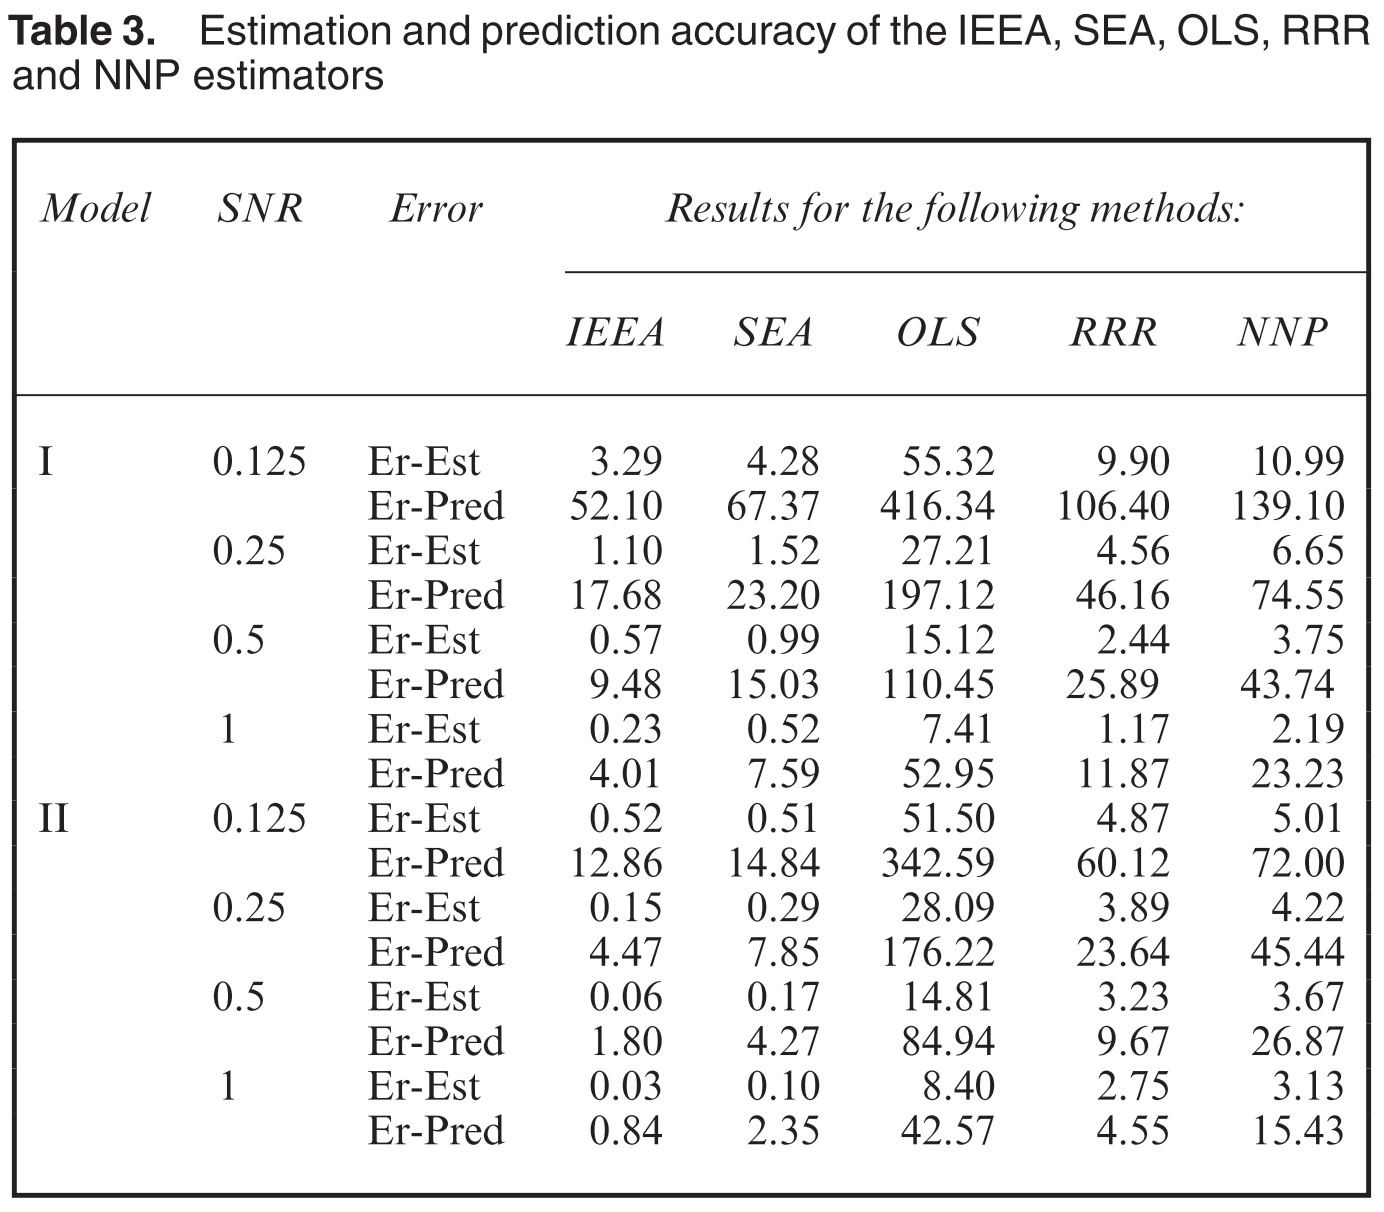
\includegraphics[scale=0.4]{tab3.png}
\end{center}
\end{frame}

\note[itemize]{
\item IEEA: proposed method; regularization parameter chosen using BIC.
\item SEA: simplification of EEA. In SEA: sequentially perform sparse unit rank regression, each time with data matrix Y replaced by residual matrix Y - X B. Has been used in many penalized matrix decomposition problems. Correspond to a different decomposition of the coefficient matrix other than SVD, and need not produce SVD layers of B, so it is not suitable for recovering the desired sparse SVD structure in B. Regularization parameter chosen using BIC.
\item OLS: least squares
\item RRR: reduced rank regression (ordinary regression but allowing for possibility that coefficient matrix is rank-deficient (e.g. two columns are identical)
\item NNP: nuclear-norm penalized regression (nuclear norm is sum of absolute values of eigenvalues)
}

\note[itemize]{
\item Model I: \(p = K = 25, n=50, r^*=3\). 
\item Model II:  \(p = K = 60, n=50, r^*=3\) (same but more noise features, and more responses even though their columns of \(B\) don't add to rank of matrix).
\item Then generate data via \(Y = XB + W\) with \(\sigma\) chosen according to desired SNR.
\item Vary SNR as well as estimation and prediction error. Er-Est: \( \lVert B^* - \hat{B} \rVert_F^2/(pq)\). Er-Pred: \( \lVert XB^* - X\hat{B} \rVert_F^2/(pq)\). 
\item We see that authors are correct that IEEA pretty much uniformly outperforms SEA, althoguh this is the second best method. (Sparsity assumption benefits method when model dimension is high and number of irrelevant responses or predictors is large.)
\item Next RRR, then NNP, finally OLS.
}

%\begin{frame}{Blocks}
%\begin{block}{Block Title}
%You can also highlight sections of your presentation in a block, with it's own title
%\end{block}
%\begin{theorem}
%There are separate environments for theorems, examples, definitions and proofs.
%\end{theorem}
%\begin{example}
%Here is an example of an example block.
%\end{example}
%\end{frame}

% Placing a * after \section means it will not show in the
% outline or table of contents.
%\section*{Summary}
%
%\begin{frame}{Summary}
%  \begin{itemize}
%  \item
%    The \alert{first main message} of your talk in one or two lines.
%  \item
%    The \alert{second main message} of your talk in one or two lines.
%  \item
%    Perhaps a \alert{third message}, but not more than that.
%  \end{itemize}
%  
%  \begin{itemize}
%  \item
%    Outlook
%    \begin{itemize}
%    \item
%      Something you haven't solved.
%    \item
%      Something else you haven't solved.
%    \end{itemize}
%  \end{itemize}
%\end{frame}



% All of the following is optional and typically not needed. 
%\appendix
%\section<presentation>*{\appendixname}
%\subsection<presentation>*{For Further Reading}
%
%\begin{frame}[allowframebreaks]
%  \frametitle<presentation>{For Further Reading}
%    
%  \begin{thebibliography}{10}
%    
%  \beamertemplatebookbibitems
%  % Start with overview books.
%
%  \bibitem{Author1990}
%    A.~Author.
%    \newblock {\em Handbook of Everything}.
%    \newblock Some Press, 1990.
% 
%    
%  \beamertemplatearticlebibitems
%  % Followed by interesting articles. Keep the list short. 
%
%  \bibitem{Someone2000}
%    S.~Someone.
%    \newblock On this and that.
%    \newblock {\em Journal of This and That}, 2(1):50--100,
%    2000.
%  \end{thebibliography}
%\end{frame}

\end{document}


